\documentclass[a4paper]{article}
\usepackage[utf8]{inputenc}
\usepackage{amsmath}
\usepackage{amssymb}
\usepackage{siunitx}
\usepackage[ngerman]{babel}
\usepackage{pgfplots}
\usepackage{hyperref}
\usepackage{pgfplotstable}
\usepackage[section]{placeins}
\usepackage{enumitem}
\usepackage{float}
\usepackage{booktabs}
\usepackage[normalem]{ulem}
\usepackage{subcaption}
\usepackage{chngpage}
\usepackage[overload]{empheq}

\pgfplotsset{compat=1.15}

% Full Reference, produces: "Abbildung 3: Schaltplan"
\newcommand*{\fullref}[1]{\hyperref[{#1}]{\autoref*{#1}: \nameref*{#1}}}

\title{GPET\\ Auswertung Versuch 8\\ Gruppe 1}

\author{Jonas Otto\\ \href{mailto:jonas@jonasotto.com}{jonas@jonasotto.com} 
   \and Luca Krüger \\ \href{mailto:luca.krueger@uni-ulm.de}{luca.krueger@uni-ulm.de} }
\date{vom 5. Juni 2018}

\begin{document}
    
\maketitle
\newpage

\section{Vorbereitende Aufgaben}

\subsection{Diodenkennlinie}
$-I_s$ verschiebt die exponentielle Kennlinie nach unten, sodass $I(0\si{V})=0\si{A}$ gilt.


\begin{eqnarray*}
    U_{Vereinfacht} \cdot 0.99 &=& U_{Ideal}\\
    0.99 &=& 1-\frac{1}{\exp{\frac{U_d}{U_t}}}\\
    \exp{\frac{U_d}{U_t}} &=& 100\\
    U_d=\ln{(100)} \cdot U_t &=& 4.6 \cdot U_t
\end{eqnarray*}

Der Fehler durch die Vereinfachung ist $>1\%$ für $U_d < 6.6 \cdot U_t$.

\subsection{Schaltung zur Messung von Kennlinien}
$R_v$ begrenzt den Strom in Durchlassrichtung.
In Sperrrichtung ist kein Widerstand zur Strombegrenzung nötig.
Der Strom $I_D$ kann über den Spannungsabfall am Widerstand bestimmt werden.

\subsection{Begrenzerschaltungen}

\[
    U_{out} = 
    \begin{cases}
        U_{in},& \text{für } -0.6\si{V} < U_{in} < 9.6\si{V}\\
        9.6\si{V},& \text{für } U_{in} > 9.6\si{V}\\
        -0.6\si{V},& \text{für } U_{in} < -0.6\si{V}
    \end{cases}
\]
Eine äquivalente Schaltung kann mit einer Zenerdiode mit entsprechender Durchbruchspannung realisiert werden, die in Sperrrichtung zu $0V$ geschaltet wird.

\subsection{Gleichrichterschaltungen}
Beim Brückengleichrichter werden beide Halbwellen gleichgerichtet, was deutlich effizienter ist als jeweils nur die positive Halbwelle zu nutzen. Ein Nachteil des Brückengleichrichter ist, dass zwei Dioden in Reihe zur Last geschaltet sind anstatt nur eine Dioder.

\newpage

\section{Versuchsauswertung}

\subsection{Versuch 1: Kennlinie Ge- und Si-Diode}

\subsubsection{Ge-Diode}

%https://tex.stackexchange.com/a/83929/143051
\begin{figure}[H]
    \centering
        \begin{tikzpicture}
            \begin{axis}[
            xlabel={$U_D [V]$},
            ylabel={$I_D [A]$}]
                \addplot table [x=u, y=I, col sep=comma, mark=none] {versuch1/ge_durchlass_calc.csv};
                \addplot table [x=u, y=I, col sep=comma, mark=none] {versuch1/ge_sperr_calc.csv};
            \end{axis}
        \end{tikzpicture}
    \caption{Kennlinie Ge-Diode}
    \label{fig:kennlinie-ge}
\end{figure}

\begin{figure}[H]
    \centering
        \begin{tikzpicture}
            \begin{axis}[
            xlabel={$U_D [V]$},
            ylabel={$I_D [A]$}]
                \addplot table [x=u, y=I, col sep=comma, mark=none] {versuch1/ge_durchlass_calc.csv};
            \end{axis}
        \end{tikzpicture}
    \caption{Kennlinie Ge-Diode, Durchlassrichtung}
    \label{fig:kennlinie-ge-durchlass}
\end{figure}

\begin{figure}[H]
    \centering
        \begin{tikzpicture}
            \begin{axis}[
            xlabel={$U_D [V]$},
            ylabel={$I_D [A]$},
            ymode=log]
                \addplot table [x=u, y=I, col sep=comma, mark=none] {versuch1/ge_durchlass_calc.csv};
            \end{axis}
        \end{tikzpicture}
    \caption{Kennlinie Ge-Diode, Durchlassrichtung, Halblogarithmisch}
    \label{fig:kennlinie-ge-durchlass-hlog}
\end{figure}

Der Emmissionskoeffizient $n$ berechnet sich durch:
\begin{equation*}
    n =\frac{U_2 - U_1}{U_T \cdot \ln{\frac{I_2}{I_1}}}
\end{equation*}
mit $U_T = 26\si{mV}$ bei Zimmertemperatur. Bei der Germaniumdiode werden die Werte $I(0.31335\si{V})=0.0009197\si{A}$ und $I(0.20487\si{V})=0.00024837\si{A}$ gewählt, aus denen sich ein Emissionskoeffizient $n=3.18$ ergibt.
Die Schwellenspannung $U_S$ beträgt $0.33\si{V}$.

\subsection{Si-Diode}

\begin{figure}[H]
    \centering
    \begin{tikzpicture}
        \begin{axis}[
        xlabel={$U_D [V]$},
        ylabel={$I_D [A]$}]
            \addplot table [x=u, y=I, col sep=comma, mark=none] {versuch1/si_durchlass_calc.csv};
            \addplot table [x=u, y=I, col sep=comma, mark=none] {versuch1/si_sperr_calc.csv};
        \end{axis}
    \end{tikzpicture}
    \caption{Kennlinie Si-Diode}
    \label{fig:kennlinie-si}
\end{figure}

%https://tex.stackexchange.com/a/83929/143051
\begin{figure}[H]
    \centering
    \begin{tikzpicture}
        \begin{axis}[
        xlabel={$U_D [V]$},
        ylabel={$I_D [A]$}]
            \addplot table [x=u, y=I, col sep=comma, mark=none] {versuch1/si_durchlass_calc.csv};
        \end{axis}
    \end{tikzpicture}
    \caption{Kennlinie Si-Diode, Durchlassrichtung}
    \label{fig:kennlinie-si-durchlass}
\end{figure}

\begin{figure}[H]
    \centering
    \begin{tikzpicture}
        \begin{axis}[
        xlabel={$U_D [V]$},
        ylabel={$I_D [A]$},
        ymode=log]
            \addplot table [x=u, y=I, col sep=comma, mark=none] {versuch1/si_durchlass_calc.csv};
        \end{axis}
    \end{tikzpicture}
    \caption{Kennlinie Si-Diode, Durchlassrichtung, Halblogarithmisch}
    \label{fig:kennlinie-si-durchlass-hlog}
\end{figure}

Bei der Siliziumdiode werden die Werte $I(0.5664\si{V})=0.0009\si{A}$ und $I(0.4358\si{V})=0.0001\si{A}$ gewählt, aus denen sich ein Emissionskoeffizient $n=2.28$ ergibt.
Die Schwellenspannung $U_S$ beträgt $0.56\si{V}$.

Die Abweichung des Emissionskoeffizienten bei der Si- und Ge-Diode zum erwarteten Wert zwischen 1 und 2 liegt daran, dass zur Berechnung sehr kleine Werte von Strom und Spannung gewählt werden sollten. Die kleinstmöglich gemessenen Werte sind offensichtlich in diesem Fall bereits so groß, dass andere Nichtidealitäten wie Bahnwiderstand und Serienwiderstand die Messung verfälschen.

Der Serienwiderstand kann nur bei kleinem Diodenstrom bestimmt werden, da bei größerem Strom der Bahnwiderstand $R_B$ für große Abweichung sorgt. Ohne $R_B$ wäre die Kennlinie in halblogarithmischer Darstellung (Abbildung \ref{fig:kennlinie-ge-durchlass-hlog} und \ref{fig:kennlinie-si-durchlass-hlog}) eine Gerade, was hier nur bei kleinen Werten gegeben ist. Die Silizium Diode scheint außerdem einen deutlich geringeren Bahnwiderstand zu haben, da die Kennlinie in halblogarithmischer Darstellung ähnlich zu einer Geraden verläuft.

Ge- und Si-Diode unterscheiden sich auch weiter in der Kennlinie. Der Strom an der Si-Diode steigt im Durchlassbereich deutlich stärker an.

\subsection{Versuch 2: Kennlinie Z-Diode}

Um die Kennlinie der Zener Diode aufzuzeichnen, kann in Durchlassrichtung die gleiche Schaltung wie zuvor verwendet werden. In Sperrrichtung muss allerdings ein Widerstand zur Strombegrenzung in Reihe geschaltet werden, da die Diode unterhalb der Durchbruchspannung wieder leitet.

\begin{figure}[H]
    \centering
    \begin{tikzpicture}
        \begin{axis}[
        xlabel={$U_D [V]$},
        ylabel={$I_D [A]$}]
            \addplot table [x=u, y=I, col sep=comma, mark=none] {versuch2/data_zener_durchlass_calc.csv};
            \addplot table [x=u, y=I, col sep=comma, mark=none] {versuch2/data_zener_sperr_calc.csv};
        \end{axis}
    \end{tikzpicture}
    \caption{Kennlinie Z-Diode}
    \label{fig:kennlinie-z}
\end{figure}

\subsection{Versuch 3: Begrenzerschaltung}

\begin{figure}[H]
    \centering
    \begin{tikzpicture}
        \begin{axis}[
        xlabel={$U_{in} [V]$},
        ylabel={$U_{out} [V]$},
        legend style={at={(0.1,0.9)},anchor=north west}]
            \addplot table [x=ue, y=uo, col sep=comma, mark=none] {versuch3/data_begrenzer.csv};
            \addlegendentry{Begrenzer}
            \addplot table [x=ue, y=uo, col sep=comma, mark=none] {versuch3/data_begrenzer_vereinfacht.csv};
            \addlegendentry{Z-Diode}
        \end{axis}
    \end{tikzpicture}
    \caption{Begrenzerschaltung}
    \label{fig:begrenzerschaltung}
\end{figure}

Diese Begrenzerschaltung oder die vereinfachte Schaltung mit Zenerdiode kann verwendet werden, um elektrische Bauteile oder Geräte vor falschen Eingangsspannungen zu schützen, welche das Gerät beschädigen könnten.

\subsection{Versuch 4: Graetz-Gleichrichter}

\paragraph{1}

Ohne Kondensator werden negative Halbwellen invertiert. Der Spannungsabfall an den zwei jeweils leitenden Dioden erklärt die Stellen zwischen den Peaks, an denen $U_{out}=0$ ist.

\begin{figure}[H]
    \centering
    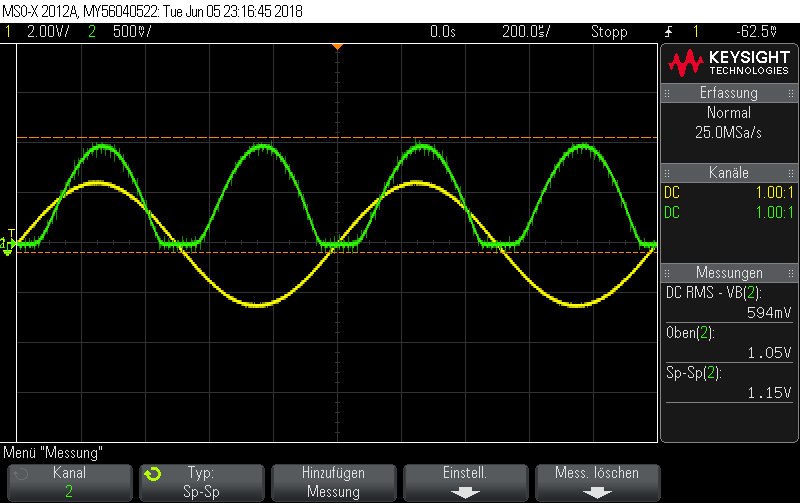
\includegraphics[width=0.8\textwidth]{versuch4/versuch4_1.png}
    \caption{$10\si{k\ohm}$, kein Kondensator}
    \label{fig:versuch4-1}
\end{figure}

\paragraph{2}

Durch Hinzufügen des Kondensators wird das Ausgangssignal geglättet. Da die Kapazität aber noch gering ist, ist das Ausgangssignal noch immer nicht konstant.

\begin{figure}[H]
    \centering
    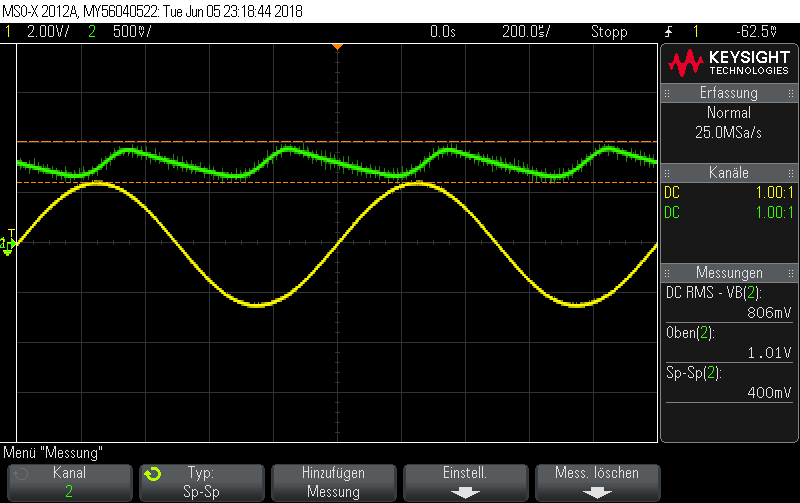
\includegraphics[width=0.8\textwidth]{versuch4/versuch4_2.png}
    \caption{$10\si{k\ohm}$, $100\si{nF}$}
    \label{fig:versuch4-2}
\end{figure}

\paragraph{3}

Durch erhöhen der Kapazität wird ein fast vollständig konstantes Ausgangssignal erreicht.

\begin{figure}[H]
    \centering
    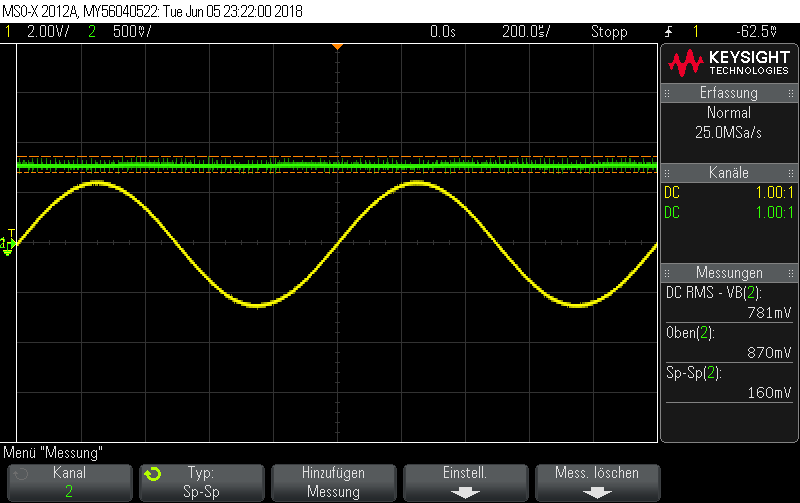
\includegraphics[width=0.8\textwidth]{versuch4/versuch4_3.png}
    \caption{$10\si{k\ohm}$, $2.2\si{\micro F}$}
    \label{fig:versuch4-3}
\end{figure}

\paragraph{4}

Durch verringern des Lastwiderstandes und dadurch erhöhen des Stroms durch den Lastwiderstand verändert sich die Impedanz der Last und es tritt wieder eine geringe Welligkeit des Ausgangssignals auf.

\begin{figure}[H]
    \centering
    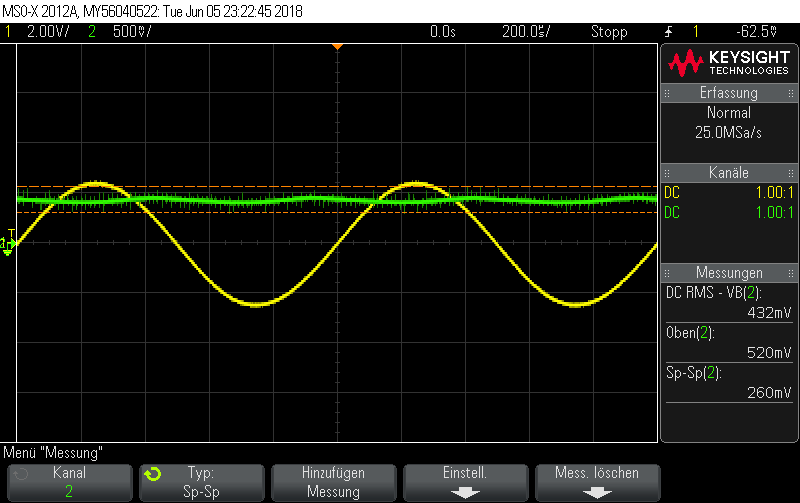
\includegraphics[width=0.8\textwidth]{versuch4/versuch4_4.png}
    \caption{$1\si{k\ohm}$, $2.2\si{\micro F}$}
    \label{fig:versuch4-4}
\end{figure}

Der Transformator kann genutzt werden, um das Bezugspotential des Ausgangs auf Masse zu legen. In unserem Versuchsaufbau wäre dies aber nicht notwendig, da das Eingangssignal aus dem Funktionsgenerator bereits die gleiche Referenz wie die Messung besitzt.

\subsection{Versuch 5: Leuchtdioden}

\begin{figure}[H]
    \centering
    \begin{tikzpicture}
        \begin{axis}[
        xlabel={$U_D [V]$},
        ylabel={$I_D [A]$}]
            \addplot table [x=u, y=I, col sep=comma, mark=none] {versuch5/data_led.csv};
        \end{axis}
    \end{tikzpicture}
    \caption{Kennlinie LED}
    \label{fig:kennlinie-led}
\end{figure}

\begin{figure}[H]
    \centering
    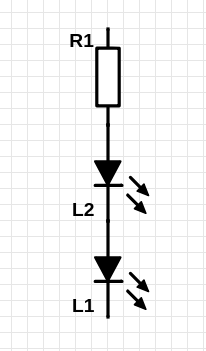
\includegraphics[height=4cm]{versuch5/leds.png}
    \caption{Reihenschaltung LEDs}
    \label{fig:leds}
\end{figure}

Die LEDs werden in Reihe mit einem Widerstand wie in Abbildung \ref{fig:leds} geschaltet um den Strom zu begrenzen. Die Schaltung wird von einer Spannungsquelle der Spannung $U=5\si{V}$ versorgt.
Bei einem Strom von $I=10\si{mA}$ fällt über den Leds jeweils eine Spannung von ungefähr $U=2\si{V}$ ab. Das heißt, über dem Vorwiderstand muss bei einem gleichen Strom genau eine Spannung von $U=1\si{V}$ abfallen. Daraus ergibt sich ein Vorwiderstand $R_1=\frac{U}{I}=100\si{\ohm}$

\end{document}